\documentclass[10pt,a4paper,final]{article}
\usepackage[utf8x]{inputenc}
\usepackage{ucs}
\usepackage[english]{babel}
\usepackage{multirow}
\usepackage{rotating}
\author{Lukáš Petrovický}
\title{RAS2012: Competition Entry}
\begin{document}

\maketitle

\begin{abstract}
This article describes an entry to the 2012 RAS Problem Solving Competition, concerning dispatching on multi-track territories. The entry is based on the Drools Planner, a Java-based solver. On a reasonably recent computer, the resulting algorithm is able to produce feasible results within a minute and has been fine-tuned to provide best results in under 3 minutes. Source code of the entry is open and well documented.
\end{abstract}

\section{Introduction}

\section{Key concepts}

In this section, we will describe the various approaches we have taken to implement the rules and constrains required by the competition. These are the key concepts leveraged in the algorithm, whose implementation will be described in later sections.

\begin{description}
\item[Train routes] From each particular data set, a territory is built. This territory is then analyzed and every possible route through that territory is found. Each train then holds a set of routes it is allowed to take, from which a solver will attempt to pick the best one\footnote{The competition rules state that the algorithm cannot assign trains to sidings. A case could be made that our approach here violates this rule. The algorithm may, indeed, explicitly put a train on a route with a siding. However, as the solution improves, this situation will inevitably be reduced to only occurring during a meet-pass event. Strictly speaking, we don't violate the rule at all, since we don't assign trains to sidings~-- we assign routes to trains.}. A train is not allowed to take a particular route when any of the following conditions hold true:

\begin{itemize}
\item Train is required to pass through a node that is not on the route. Examples would include situations when the route doesn't include the node with a schedule adherence requirement attached.
\item Length of the train is bigger than the length of any one siding on the route.
\item There are sidings on the route of a train carrying hazardous materials.
\item There are sidings on the route of a heavy train. This is the easiest way to fulfill the requirement that a heavy train must never use a siding when meet-passing another train.
\end{itemize}

\item[Train wait points] Our solution only allows trains to stop at specific points on the route, called ``wait points''\footnote{If we allowed the train to stop at any node on the route, we would be significantly extending the state space of the solution. We believe that it wouldn't be beneficial to the quality of the resolved system and have therefore made a decision to only stop the trains where they don't block main tracks.}. A train can be held when its lead engine enters a node for which any of the following conditions holds true:

\begin{itemize}
\item The node is the source terminal of the train. The train is not in the territory yet.
\item The node is the starting node of a crossover arc, keeping the other main track available for whatever trains to pass.
\item The node is the ending node of a siding arc. The train occupies the siding.
\end{itemize}

Trains are automatically stopped for maintenance windows. However, no additional delays are allowed in those nodes~-- the train starts to move immediately after the maintenance window is over.

\item[Train wait times] In each of the wait points described above, the algorithm may incur one of a selection of delays. These delays are called ``wait times'' and range from 1 minute to $X$ minutes, where $X$ is the minimal possible delay that would cause the train to fall outside the planning horizon waiting\footnote{This is done to once again reduce the state space by eliminating wait times that aren't viable. Once a train falls out of the planning horizon, we no longer care about its further journey.}. The wait times aren't distributed evenly across the stated range~-- they get sparser as we progress towards bigger numbers in the range. That should allow for both fine-grained and coarse-grained planning.

\item[Itinerary] An itinerary of a train consists of a route and 0 or more wait times at the wait points on that route.

\item[Solution] A solution is a set of itineraries, one for each train. The best found solution becomes a resolved system. A solution differs from the other by either of the trains taking a different route, waiting at different points and/or for different times.

\item[Conflicts] The itinerary of each train is reached separately, without accounting for the whereabouts of any other train in the territory. This inevitably leads to solutions where two trains leverage the same part of the track at the same time, thus effectively colliding. These events are called ``conflicts'' and are treated as hard constraints~-- no feasible solution will ever demonstrate any conflict\footnote{We would think it goes without saying. However, we've been getting that question over and over when describing the algorithm to friends and colleagues. Hence the clarification.}. The same goes for the mandatory time lapse between any two trains.

\end{description}

\section{Implementation}

In this section, we will describe the implementation of the algorithm, its various properties, strength and drawbacks.

\subsection{Drools Planner} 

Drools Planner\footnote{The Drools project, http://www.jboss.org/drools/} is an open-source Java-based solver that currently implements various tabu search techniques and simulated annealing. It allows for declaratively stating your problem, using the following basic concepts:

\begin{description}
\item[Planning entity] The entity used for planning, in our case it is the itinerary for a particular train.

\item[Planning variable] Each planning entity hold various variables. By changing their values, Planner can arrive at a better or worse solution. In our case, planning variables are the route for the train and wait times in wait points.

\item[Planning values] Each variable has a list of values applicable at the given point in time. For example, the itinerary has a list of routes that are available for its train to take. Each of them can become a value of the planning variable, resulting in a change in solution quality.

\item[Move] is a way to change one solution into another, to cross from one state to another in a state space. Usually a move consists of changing the value of a planning variable. In our case, we know the following moves:

\item[Scoring function] is a means of evaluating the quality of the solution. In our case, it contains of two parts~-- a hard score, representing the number of conflicts (see above), and a soft score, representing the cost of the system.

Scoring function in Planner can take two forms - first, you can write it in plain old Java. Alternatively, you can leverage Drools Expert, giving at your disposal the full power of a ReteOO-based inference engine. We use the former.

\end{description}

When all these are provided to Planner, along with a solver configuration where we specify  the types of algorithms to use\footnote{Such as simulated annealing, entity tabu, solution tabu etc.} and termination conditions, it will start traversing the state space by trying the moves, looking for the best solution. While solving, Planner makes no I/O operations, utilizing only the CPU and RAM~-- which means that any performance improvement to the scoring function, the moves or to Planner itself will directly affect the quality of your scores. 

One of the benefits of Planner is that it is a Java application. That means neither the developer of the solver nor its user is limited to any particular operating system or platform. For our development and testing, we've been using Linux, but we've seen the submission perform on Windows as well.

At the moment, Planner is a single-threaded application. Using multi-core CPUs will yield no benefit performance-wise, although you can leverage them to run multiple solvers at once~-- resolving one data set per core.

\subsection{Typical flow of the algorithm}

\begin{enumerate}
\item Start processing.
\item Parse the data set, re-constructing the territory.
\item Turn the data set into an initial solution. Each train is assigned the fastest possible route through the territory with no wait times. 
\item Launch the solver with the initial solution. The solver then iterates:

\begin{enumerate}
\item Generate all possible moves for the solution.
\item Based on the user-specified solver configuration, some or all of the moves are evaluated. This is where the simulated annealing and tabu searches come into play.
\item Should a better solution be found, store it.
\item Repeat.
\end{enumerate}

\item When a user-specified termination condition is reached, the solver ends and reports the best found solution. The termination condition in our case is 3 minutes of run time.
\item We take the solution and convert it into the submission format. Optionally, we visualize and tabulate.
\item End processing.
\end{enumerate}

\subsection{Additional features} 

During the development, debugging and tuning of the algorithm, we have developed various tools to make our work easier\footnote{As a side note, although technically not a ``feature,'' the algorithm is written in such a way that it should be very easy to adapt it for changing circumstances. For example, changing the territory to a directed graph by introducing one-way arcs should only take a couple minutes and shouldn't affect performance.}. Following is a list of them.

\begin{description}

\item[Data set parser] is generated on-the-fly from a JavaCC-based\footnote{JavaCC parser/scanner generator, http://javacc.java.net/} grammar and can be easily extended or reused in other applications.

\item[Basic visualizations] of train routes, territories and solutions are possible. We draw graphs of these to help with the analysis of the resolved systems and debugging of the algorithm.

\item[Solution validation] for reading the resolved system's XML, calculating its cost and also visualizing it. Can be used for comparing various competition submissions against each other using a single algorithm.

\end{description}


\subsection{Usage}

\subsubsection{Compiling}

We've relied on the industry-standard Maven\footnote{Apache Maven, http://maven.apache.org/} build tool for our dependency management and release needs. It is open-source and available for every major operating system. Our source code is tracked on Github\footnote{Our homepage, http://triceo.github.com/ras12/} using the Git SCM.

Once you have downloaded the Git and Maven tools, download the source code by executing the command (see Figure \ref{figure:git}). This will create a \texttt{ras12} folder in your current working directory, containing a one-for-one copy of our entire code repository. After switching into it, simply type another command (see Figure \ref{figure:maven}).

Maven starts downloading our dependencies, building our code and running our extensive tests. It may take a while and it should end in success. When it's done, switch to a directory called \texttt{ras2012-solver}. You will notice a new file called \texttt{target/ras2012-solver-1.0-jar-with-dependencies.jar}. You can use it to run the solver, as described in the following section.

\begin{figure}
\centering
\texttt{git clone git://git@github.com:triceo/ras12.git}
\caption{Obtaining the source code.}
\label{figure:git}
\end{figure}

\begin{figure}
\centering
\texttt{mvn install}
\caption{Building the binary distribution.}
\label{figure:maven}
\end{figure}

\begin{figure}
\centering
\texttt{java -jar <JAR-FILE> -r -d <PATH-TO-DATA-SET>}
\caption{Running the application in a resolver mode.}
\label{figure:run-resolver}
\end{figure}

\begin{figure}
\centering
\texttt{java -jar <JAR-FILE> -r -d <PATH-TO-DATA-SET> -x <SEED>}
\caption{Running the application in a resolver mode, specifying a random seed.}
\label{figure:run-resolver-seed}
\end{figure}

\begin{figure}
\centering
\texttt{java -jar <JAR-FILE> -e -d <PATH-TO-DATA-SET> -s <PATH-TO-XML>}
\caption{Running the application in an evaluation mode.}
\label{figure:run-evaluation}
\end{figure}

\begin{figure}
\centering
\texttt{java -jar <JAR-FILE> -l}
\caption{Running the application in lookup mode.}
\label{figure:run-lookup}
\end{figure}

\subsubsection{Running}

To start resolving a data set with a fresh random seed, see Figure \ref{figure:run-resolver}. To provide a specific random seed, see Figure \ref{figure:run-resolver-seed}.

To calculate cost for a specific resolved system, see Figure \ref{figure:run-evaluation}.

To verify how your solver configuration performs on the three provided data sets, see Figure \ref{figure:run-lookup}. It will run the algorithm many times with a fresh random seed each time and provide a summary of the results, much like in Table \ref{table:result} and Figure \ref{figure:plot}.

Please note that in all the figures, \texttt{<JAR-FILE>} refers to the \texttt{.jar} file from the previous section.

\section{Achieved results}

Running the algorithm 50 times over each data set and using a fresh random seed every time, we have compiled a set of results, see Table \ref{table:result}. All these were reached within 3 minutes in a single-threaded run, using Intel i7 Q820 processor running Fedora 17 and 2 GB of heap space inside Java 7 runtime environment.

\begin{table}
\footnotesize
\caption{Submission performance per data set.}
\centering
\begin{tabular}{c||c|c|c|c|c}
\hline \hline
                 & Best                 & Q1                 & Q2                & Q3                & Worst \\ 
\hline
TOY & \$1074   & \$1074   & \$1074  & \$1074  & \$1074 \\
\hline
RDS1 & \$2056   & \$2251   & \$2561.5  & \$3385  & \$4628 \\
\hline
RDS2 & \$7895   & \$9270   & \$9851.5  & \$10600  & \$12462 \\
\hline
RDS3 & \$10257   & \$11194   & \$11816  & \$12396  & \$14135 \\
\end{tabular} 
\label{table:result} 
\end{table}

\begin{figure}
\centering
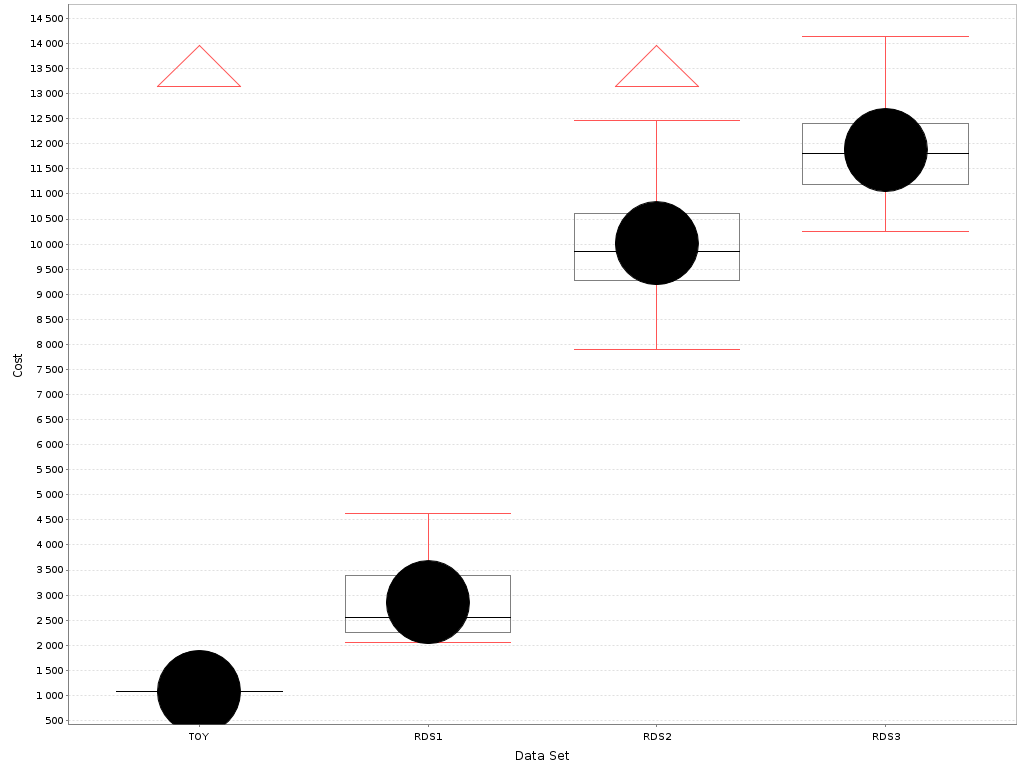
\includegraphics[width=120mm]{chart.png}
\caption{Plotting the data for the various resolved systems.}
\label{figure:plot}
\end{figure}

Please note that via the benchmarking functionality of Drools Planner, users may be able to fine-tune the algorithm to be focused either on providing better solutions or on faster turnaround times. Drools Planner even allows for retrieving the intermediate results of the algorithm and modifying the problem while it's being solved, which makes it the ideal tool for real-time planning.

For statistics of the resolved systems, see tables \ref{table:RASDATASET1}, \ref{table:RASDATASET2} and \ref{table:RASDATASET3} respectively. 

\section{Conclusion}

We are submitting a well-documented solution to the stated problem which handles data sets both large and small, is easy to understand and extend and doesn't limit the user to any particular computing platform. We allow for tabulating and visualizing resolved systems for easier analysis, be they ours or competitors'.

The submission is configured to work reasonably well on all three provided data sets. Users in the real world are encouraged to benchmark various solver configurations to come up with the one that matches the scale of their particular problem.

\appendix

Following are appendixes where we provide statistics of the best available resolved systems. The paper would be complete even without them, for which reason we believe they shouldn't be counted toward the 10-page limit.

\section{Resolved systems}

In this section, we show the best solutions reached for each data set. 

\begin{sidewaystable}
\footnotesize
\caption{Resolved system ``RAS DATA SET 1'', costing \$1199. Seed: 3458425443814323529.}
\centering
\begin{tabular}{c||c|c|c||c|c|c|c||c|c|c}
  \hline \hline
  &
  Unpref. & 
  Delay &
  Pty &
  Node &
  SA &
  Actual &
  Pty &
  TWT &
  Actual &
  Pty \\
      \hline
      \multirow{2}{*}{A1} &
      \multirow{2}{*}{0} &
      \multirow{2}{*}{0} &
      \multirow{2}{*}{0} &
      37 &
      3600 &
        3172.5 &
        0 &
      \multirow{2}{*}{5400} &
        \multirow{2}{*}{6106.5} &
        \multirow{2}{*}{0}
      \\
      \cline{5-8}
       &
       &
       &
       &
      39 &
      7800 &
        6106.5 &
        0 &
      
         &
        
      \\
      \hline
      \multirow{2}{*}{A2} &
      \multirow{2}{*}{0} &
      \multirow{2}{*}{1800} &
      \multirow{2}{*}{300} &
      37 &
      7800 &
        7924.742 &
        0 &
      \multirow{2}{*}{9000} &
        \multirow{2}{*}{10602.01} &
        \multirow{2}{*}{0}
      \\
      \cline{5-8}
       &
       &
       &
       &
      39 &
      12000 &
        10602.01 &
        0 &
      
         &
        
      \\
      \hline
      \multirow{2}{*}{B1} &
      \multirow{2}{*}{12} &
      \multirow{2}{*}{0} &
      \multirow{2}{*}{0} &
      37 &
      12600 &
        10947.271 &
        0 &
      \multirow{2}{*}{13800} &
        \multirow{2}{*}{14414.255} &
        \multirow{2}{*}{0}
      \\
      \cline{5-8}
       &
       &
       &
       &
      0 &
      17400 &
        14414.255 &
        0 &
      
         &
        
      \\
      \hline
      \multirow{2}{*}{B2} &
      \multirow{2}{*}{4} &
      \multirow{2}{*}{2160} &
      \multirow{2}{*}{300} &
      37 &
      15600 &
        16424.466 &
        0 &
      \multirow{2}{*}{16800} &
        \multirow{2}{*}{19520.46} &
        \multirow{2}{*}{0}
      \\
      \cline{5-8}
       &
       &
       &
       &
      39 &
      19800 &
        19520.46 &
        0 &
      
         &
        
      \\
      \hline
      \multirow{2}{*}{B3} &
      \multirow{2}{*}{0} &
      \multirow{2}{*}{1560} &
      \multirow{2}{*}{216} &
      37 &
      40200 &
        41027.661 &
        0 &
      \multirow{2}{*}{42000} &
        \multicolumn{2}{c}{\multirow{2}{*}{N/A}}
      \\
      \cline{5-8}
       &
       &
       &
       &
      39 &
      45000 &
        \multicolumn{2}{|c||}{N/A} &
      
        
      \\
      \hline
      \multirow{2}{*}{C1} &
      \multirow{2}{*}{0} &
      \multirow{2}{*}{0} &
      \multirow{2}{*}{0} &
      37 &
      19200 &
        18294 &
        0 &
      \multirow{2}{*}{21600} &
        \multirow{2}{*}{21666} &
        \multirow{2}{*}{0}
      \\
      \cline{5-8}
       &
       &
       &
       &
      39 &
      24600 &
        21666 &
        0 &
      
         &
        
      \\
      \hline
      \multirow{2}{*}{C2} &
      \multirow{2}{*}{0} &
      \multirow{2}{*}{0} &
      \multirow{2}{*}{0} &
      37 &
      27000 &
        25026.431 &
        0 &
      \multirow{2}{*}{28800} &
        \multirow{2}{*}{28634.147} &
        \multirow{2}{*}{0}
      \\
      \cline{5-8}
       &
       &
       &
       &
      39 &
      33000 &
        28634.147 &
        0 &
      
         &
        
      \\
      \hline
      \multirow{2}{*}{D1} &
      \multirow{2}{*}{6} &
      \multirow{2}{*}{2580} &
      \multirow{2}{*}{215} &
      37 &
      29400 &
        28914.852 &
        0 &
      \multirow{2}{*}{31200} &
        \multirow{2}{*}{33483.416} &
        \multirow{2}{*}{0}
      \\
      \cline{5-8}
       &
       &
       &
       &
      0 &
      36600 &
        33483.416 &
        0 &
      
         &
        
      \\
      \hline
      \multirow{2}{*}{D2} &
      \multirow{2}{*}{14} &
      \multirow{2}{*}{1320} &
      \multirow{2}{*}{110} &
      37 &
      21600 &
        20536.749 &
        0 &
      \multirow{2}{*}{23400} &
        \multirow{2}{*}{25262.176} &
        \multirow{2}{*}{0}
      \\
      \cline{5-8}
       &
       &
       &
       &
      0 &
      28200 &
        25262.176 &
        0 &
      
         &
        
      \\
      \hline
      \multirow{2}{*}{D3} &
      \multirow{2}{*}{22} &
      \multirow{2}{*}{0} &
      \multirow{2}{*}{0} &
      37 &
      35400 &
        33325.717 &
        0 &
      \multirow{2}{*}{37200} &
        \multirow{2}{*}{37464.618} &
        \multirow{2}{*}{0}
      \\
      \cline{5-8}
       &
       &
       &
       &
      0 &
      41400 &
        37464.618 &
        0 &
      
         &
        
      \\
      \hline
      \multirow{2}{*}{E1} &
      \multirow{2}{*}{0} &
      \multirow{2}{*}{0} &
      \multirow{2}{*}{0} &
      37 &
      36000 &
        34047 &
        0 &
      \multirow{2}{*}{39000} &
        \multirow{2}{*}{39339} &
        \multirow{2}{*}{0}
      \\
      \cline{5-8}
       &
       &
       &
       &
      39 &
      44400 &
        39339 &
        0 &
      
         &
        
      \\
      \hline
      \multirow{2}{*}{F1} &
      \multirow{2}{*}{0} &
      \multirow{2}{*}{0} &
      \multirow{2}{*}{0} &
      37 &
      57600 &
        \multicolumn{2}{|c||}{N/A} &
      \multirow{2}{*}{63000} &
        \multicolumn{2}{c}{\multirow{2}{*}{N/A}}
      \\
      \cline{5-8}
       &
       &
       &
       &
      0 &
      75000 &
        \multicolumn{2}{|c||}{N/A} &
      
        
      \\
\end{tabular}
\label{table:RASDATASET1} 
\end{sidewaystable}

\begin{sidewaystable}
\footnotesize
\caption{Resolved system ``RAS DATA SET 2'', costing \$7955. Seed: 3842188991823749668.}
\centering
\begin{tabular}{c||c|c|c||c|c|c|c||c|c|c}
  \hline \hline
  &
  Unpref. & 
  Delay &
  Pty &
  Node &
  SA &
  Actual &
  Pty &
  TWT &
  Actual &
  Pty \\
      \hline
      \multirow{2}{*}{A1} &
      \multirow{2}{*}{0} &
      \multirow{2}{*}{4860} &
      \multirow{2}{*}{810} &
      37 &
      3600 &
        7942.5 &
        0 &
      \multirow{2}{*}{5400} &
        \multirow{2}{*}{10489.5} &
        \multirow{2}{*}{0}
      \\
      \cline{5-8}
       &
       &
       &
       &
      39 &
      7800 &
        10489.5 &
        0 &
      
         &
        
      \\
      \hline
      \multirow{2}{*}{A2} &
      \multirow{2}{*}{0} &
      \multirow{2}{*}{0} &
      \multirow{2}{*}{0} &
      37 &
      11400 &
        9724.742 &
        0 &
      \multirow{2}{*}{12600} &
        \multirow{2}{*}{13163.692} &
        \multirow{2}{*}{0}
      \\
      \cline{5-8}
       &
       &
       &
       &
      39 &
      15600 &
        13163.692 &
        0 &
      
         &
        
      \\
      \hline
      \multirow{2}{*}{A3} &
      \multirow{2}{*}{0} &
      \multirow{2}{*}{0} &
      \multirow{2}{*}{0} &
      37 &
      18000 &
        17185.5 &
        0 &
      \multirow{2}{*}{19800} &
        \multirow{2}{*}{19732.5} &
        \multirow{2}{*}{0}
      \\
      \cline{5-8}
       &
       &
       &
       &
      39 &
      22200 &
        19732.5 &
        0 &
      
         &
        
      \\
      \hline
      \multirow{2}{*}{A4} &
      \multirow{2}{*}{7} &
      \multirow{2}{*}{0} &
      \multirow{2}{*}{0} &
      37 &
      31800 &
        35560.967 &
        0 &
      \multirow{2}{*}{39000} &
        \multirow{2}{*}{38809.634} &
        \multirow{2}{*}{0}
      \\
      \cline{5-8}
       &
       &
       &
       &
      0 &
      36600 &
        38809.634 &
        0 &
      
         &
        
      \\
      \hline
      \multirow{2}{*}{B1} &
      \multirow{2}{*}{9} &
      \multirow{2}{*}{780} &
      \multirow{2}{*}{108} &
      37 &
      4800 &
        6421.758 &
        0 &
      \multirow{2}{*}{9600} &
        \multirow{2}{*}{10918.224} &
        \multirow{2}{*}{0}
      \\
      \cline{5-8}
       &
       &
       &
       &
      39 &
      9000 &
        10918.224 &
        0 &
      
         &
        
      \\
      \hline
      \multirow{2}{*}{B2} &
      \multirow{2}{*}{0} &
      \multirow{2}{*}{0} &
      \multirow{2}{*}{0} &
      37 &
      26400 &
        32155.875 &
        0 &
      \multirow{2}{*}{35400} &
        \multirow{2}{*}{35679.375} &
        \multirow{2}{*}{0}
      \\
      \cline{5-8}
       &
       &
       &
       &
      39 &
      31200 &
        35679.375 &
        0 &
      
         &
        
      \\
      \hline
      \multirow{2}{*}{B3} &
      \multirow{2}{*}{0} &
      \multirow{2}{*}{15357.855} &
      \multirow{2}{*}{2133} &
      37 &
      11400 &
        22527 &
        218 &
      \multirow{2}{*}{10800} &
        \multirow{2}{*}{25953.431} &
        \multirow{2}{*}{90}
      \\
      \cline{5-8}
       &
       &
       &
       &
      0 &
      16800 &
        25953.431 &
        108 &
      
         &
        
      \\
      \hline
      \multirow{2}{*}{C1} &
      \multirow{2}{*}{16} &
      \multirow{2}{*}{0} &
      \multirow{2}{*}{0} &
      37 &
      26400 &
        36093.005 &
        138 &
      \multirow{2}{*}{39000} &
        \multirow{2}{*}{39657.47} &
        \multirow{2}{*}{0}
      \\
      \cline{5-8}
       &
       &
       &
       &
      39 &
      31800 &
        39657.47 &
        36 &
      
         &
        
      \\
      \hline
      \multirow{2}{*}{C2} &
      \multirow{2}{*}{5} &
      \multirow{2}{*}{0} &
      \multirow{2}{*}{0} &
      37 &
      0 &
        198 &
        0 &
      \multirow{2}{*}{3600} &
        \multirow{2}{*}{4374} &
        \multirow{2}{*}{0}
      \\
      \cline{5-8}
       &
       &
       &
       &
      39 &
      5400 &
        4374 &
        0 &
      
         &
        
      \\
      \hline
      \multirow{2}{*}{C3} &
      \multirow{2}{*}{23} &
      \multirow{2}{*}{1920} &
      \multirow{2}{*}{213} &
      37 &
      20400 &
        23527.716 &
        0 &
      \multirow{2}{*}{25200} &
        \multirow{2}{*}{27537.861} &
        \multirow{2}{*}{0}
      \\
      \cline{5-8}
       &
       &
       &
       &
      0 &
      25800 &
        27537.861 &
        0 &
      
         &
        
      \\
      \hline
      \multirow{2}{*}{D1} &
      \multirow{2}{*}{0} &
      \multirow{2}{*}{2400} &
      \multirow{2}{*}{200} &
      37 &
      43800 &
        43015.5 &
        0 &
      \multirow{2}{*}{44400} &
        \multicolumn{2}{c}{\multirow{2}{*}{N/A}}
      \\
      \cline{5-8}
       &
       &
       &
       &
      39 &
      51000 &
        \multicolumn{2}{|c||}{N/A} &
      
        
      \\
      \hline
      \multirow{2}{*}{D2} &
      \multirow{2}{*}{0} &
      \multirow{2}{*}{0} &
      \multirow{2}{*}{0} &
      37 &
      3600 &
        2179.383 &
        0 &
      \multirow{2}{*}{6600} &
        \multirow{2}{*}{6383.07} &
        \multirow{2}{*}{0}
      \\
      \cline{5-8}
       &
       &
       &
       &
      39 &
      9600 &
        6383.07 &
        0 &
      
         &
        
      \\
      \hline
      \multirow{2}{*}{E1} &
      \multirow{2}{*}{0} &
      \multirow{2}{*}{0} &
      \multirow{2}{*}{0} &
      37 &
      6600 &
        4652.184 &
        0 &
      \multirow{2}{*}{9600} &
        \multirow{2}{*}{9224.186} &
        \multirow{2}{*}{0}
      \\
      \cline{5-8}
       &
       &
       &
       &
      39 &
      14400 &
        9224.186 &
        0 &
      
         &
        
      \\
      \hline
      \multirow{2}{*}{E2} &
      \multirow{2}{*}{8} &
      \multirow{2}{*}{10740} &
      \multirow{2}{*}{447} &
      37 &
      1800 &
        11874.858 &
        0 &
      \multirow{2}{*}{7200} &
        \multirow{2}{*}{18290.006} &
        \multirow{2}{*}{6}
      \\
      \cline{5-8}
       &
       &
       &
       &
      0 &
      10800 &
        18290.006 &
        0 &
      
         &
        
      \\
      \hline
      \multirow{2}{*}{E3} &
      \multirow{2}{*}{0} &
      \multirow{2}{*}{40920} &
      \multirow{2}{*}{1705} &
      37 &
      9000 &
        \multicolumn{2}{|c||}{N/A} &
      \multirow{2}{*}{12000} &
        \multicolumn{2}{c}{\multirow{2}{*}{N/A}}
      \\
      \cline{5-8}
       &
       &
       &
       &
      0 &
      18000 &
        \multicolumn{2}{|c||}{N/A} &
      
        
      \\
      \hline
      \multirow{2}{*}{E4} &
      \multirow{2}{*}{16} &
      \multirow{2}{*}{0} &
      \multirow{2}{*}{0} &
      37 &
      30000 &
        27107.534 &
        0 &
      \multirow{2}{*}{32400} &
        \multirow{2}{*}{32523.196} &
        \multirow{2}{*}{0}
      \\
      \cline{5-8}
       &
       &
       &
       &
      0 &
      37800 &
        32523.196 &
        0 &
      
         &
        
      \\
      \hline
      \multirow{2}{*}{F1} &
      \multirow{2}{*}{0} &
      \multirow{2}{*}{25140} &
      \multirow{2}{*}{698} &
      37 &
      29400 &
        \multicolumn{2}{|c||}{N/A} &
      \multirow{2}{*}{33600} &
        \multicolumn{2}{c}{\multirow{2}{*}{N/A}}
      \\
      \cline{5-8}
       &
       &
       &
       &
      39 &
      41400 &
        \multicolumn{2}{|c||}{N/A} &
      
        
      \\
      \hline
      \multirow{2}{*}{F2} &
      \multirow{2}{*}{0} &
      \multirow{2}{*}{34620} &
      \multirow{2}{*}{961} &
      37 &
      30000 &
        \multicolumn{2}{|c||}{N/A} &
      \multirow{2}{*}{36000} &
        \multicolumn{2}{c}{\multirow{2}{*}{N/A}}
      \\
      \cline{5-8}
       &
       &
       &
       &
      0 &
      51000 &
        \multicolumn{2}{|c||}{N/A} &
      
        
      \\
\end{tabular}
\label{table:RASDATASET2} 
\end{sidewaystable}

\begin{sidewaystable}
\footnotesize
\caption{Resolved system ``RAS DATA SET 3'', costing \$11306. Seed: 9087099929377852117.}
\centering
\begin{tabular}{c||c|c|c||c|c|c|c||c|c|c}
  \hline \hline
  &
  Unpref. & 
  Delay &
  Pty &
  Node &
  SA &
  Actual &
  Pty &
  TWT &
  Actual &
  Pty \\
      \hline
      \multirow{2}{*}{A1} &
      \multirow{2}{*}{0} &
      \multirow{2}{*}{0} &
      \multirow{2}{*}{0} &
      37 &
      2400 &
        967.5 &
        0 &
      \multirow{2}{*}{4200} &
        \multirow{2}{*}{3901.5} &
        \multirow{2}{*}{0}
      \\
      \cline{5-8}
       &
       &
       &
       &
      39 &
      6000 &
        3901.5 &
        0 &
      
         &
        
      \\
      \hline
      \multirow{2}{*}{A2} &
      \multirow{2}{*}{0} &
      \multirow{2}{*}{1620} &
      \multirow{2}{*}{270} &
      37 &
      2400 &
        1165.715 &
        0 &
      \multirow{2}{*}{4200} &
        \multirow{2}{*}{5567.148} &
        \multirow{2}{*}{0}
      \\
      \cline{5-8}
       &
       &
       &
       &
      0 &
      6600 &
        5567.148 &
        0 &
      
         &
        
      \\
      \hline
      \multirow{2}{*}{A3} &
      \multirow{2}{*}{7} &
      \multirow{2}{*}{0} &
      \multirow{2}{*}{0} &
      37 &
      22800 &
        21013.718 &
        0 &
      \multirow{2}{*}{24000} &
        \multirow{2}{*}{24495.436} &
        \multirow{2}{*}{0}
      \\
      \cline{5-8}
       &
       &
       &
       &
      0 &
      27000 &
        24495.436 &
        0 &
      
         &
        
      \\
      \hline
      \multirow{2}{*}{A4} &
      \multirow{2}{*}{0} &
      \multirow{2}{*}{9900} &
      \multirow{2}{*}{1650} &
      37 &
      33600 &
        \multicolumn{2}{|c||}{N/A} &
      \multirow{2}{*}{39000} &
        \multicolumn{2}{c}{\multirow{2}{*}{N/A}}
      \\
      \cline{5-8}
       &
       &
       &
       &
      0 &
      38400 &
        \multicolumn{2}{|c||}{N/A} &
      
        
      \\
      \hline
      \multirow{2}{*}{A5} &
      \multirow{2}{*}{0} &
      \multirow{2}{*}{4815} &
      \multirow{2}{*}{802} &
      37 &
      32400 &
        36697.5 &
        0 &
      \multirow{2}{*}{34200} &
        \multirow{2}{*}{39244.5} &
        \multirow{2}{*}{0}
      \\
      \cline{5-8}
       &
       &
       &
       &
      39 &
      36600 &
        39244.5 &
        0 &
      
         &
        
      \\
      \hline
      \multirow{1}{*}{B1} &
      \multirow{1}{*}{0} &
      \multirow{1}{*}{0} &
      \multirow{1}{*}{0} &
      0 &
      1800 &
        1486.284 &
        0 &
      \multirow{1}{*}{1200} &
        \multirow{1}{*}{1486.284} &
        \multirow{1}{*}{0}
      \\
      \hline
      \multirow{1}{*}{B2} &
      \multirow{1}{*}{0} &
      \multirow{1}{*}{0} &
      \multirow{1}{*}{0} &
      39 &
      4800 &
        2869.163 &
        0 &
      \multirow{1}{*}{3000} &
        \multirow{1}{*}{2869.163} &
        \multirow{1}{*}{0}
      \\
      \hline
      \multirow{2}{*}{B3} &
      \multirow{2}{*}{0} &
      \multirow{2}{*}{1140} &
      \multirow{2}{*}{158} &
      37 &
      -3000 &
        4087.488 &
        0 &
      \multirow{2}{*}{6000} &
        \multirow{2}{*}{7060.391} &
        \multirow{2}{*}{0}
      \\
      \cline{5-8}
       &
       &
       &
       &
      39 &
      1800 &
        7060.391 &
        0 &
      
         &
        
      \\
      \hline
      \multirow{2}{*}{B4} &
      \multirow{2}{*}{0} &
      \multirow{2}{*}{18000} &
      \multirow{2}{*}{2500} &
      37 &
      16800 &
        \multicolumn{2}{|c||}{N/A} &
      \multirow{2}{*}{32400} &
        \multicolumn{2}{c}{\multirow{2}{*}{N/A}}
      \\
      \cline{5-8}
       &
       &
       &
       &
      0 &
      21600 &
        \multicolumn{2}{|c||}{N/A} &
      
        
      \\
      \hline
      \multirow{1}{*}{C1} &
      \multirow{1}{*}{0} &
      \multirow{1}{*}{6360} &
      \multirow{1}{*}{706} &
      0 &
      6000 &
        9938.568 &
        0 &
      \multirow{1}{*}{4200} &
        \multirow{1}{*}{9938.568} &
        \multirow{1}{*}{0}
      \\
      \hline
      \multirow{2}{*}{C2} &
      \multirow{2}{*}{11} &
      \multirow{2}{*}{1680} &
      \multirow{2}{*}{186} &
      37 &
      0 &
        5443.288 &
        0 &
      \multirow{2}{*}{7200} &
        \multirow{2}{*}{9051.004} &
        \multirow{2}{*}{0}
      \\
      \cline{5-8}
       &
       &
       &
       &
      39 &
      6000 &
        9051.004 &
        0 &
      
         &
        
      \\
      \hline
      \multirow{2}{*}{C3} &
      \multirow{2}{*}{0} &
      \multirow{2}{*}{14400} &
      \multirow{2}{*}{1600} &
      37 &
      30000 &
        \multicolumn{2}{|c||}{N/A} &
      \multirow{2}{*}{37200} &
        \multicolumn{2}{c}{\multirow{2}{*}{N/A}}
      \\
      \cline{5-8}
       &
       &
       &
       &
      0 &
      36000 &
        \multicolumn{2}{|c||}{N/A} &
      
        
      \\
      \hline
      \multirow{2}{*}{D1} &
      \multirow{2}{*}{13} &
      \multirow{2}{*}{1920} &
      \multirow{2}{*}{159} &
      37 &
      4200 &
        5933.996 &
        0 &
      \multirow{2}{*}{7800} &
        \multirow{2}{*}{9874.607} &
        \multirow{2}{*}{0}
      \\
      \cline{5-8}
       &
       &
       &
       &
      39 &
      10200 &
        9874.607 &
        0 &
      
         &
        
      \\
      \hline
      \multirow{2}{*}{D2} &
      \multirow{2}{*}{8} &
      \multirow{2}{*}{0} &
      \multirow{2}{*}{0} &
      37 &
      42000 &
        40013.996 &
        0 &
      \multirow{2}{*}{43800} &
        \multicolumn{2}{c}{\multirow{2}{*}{N/A}}
      \\
      \cline{5-8}
       &
       &
       &
       &
      39 &
      48000 &
        \multicolumn{2}{|c||}{N/A} &
      
        
      \\
      \hline
      \multirow{2}{*}{E1} &
      \multirow{2}{*}{0} &
      \multirow{2}{*}{43200} &
      \multirow{2}{*}{1800} &
      37 &
      10200 &
        \multicolumn{2}{|c||}{N/A} &
      \multirow{2}{*}{13200} &
        \multicolumn{2}{c}{\multirow{2}{*}{N/A}}
      \\
      \cline{5-8}
       &
       &
       &
       &
      0 &
      19200 &
        \multicolumn{2}{|c||}{N/A} &
      
        
      \\
      \hline
      \multirow{2}{*}{E2} &
      \multirow{2}{*}{26} &
      \multirow{2}{*}{4554} &
      \multirow{2}{*}{189} &
      37 &
      18000 &
        18717 &
        0 &
      \multirow{2}{*}{21000} &
        \multirow{2}{*}{25659} &
        \multirow{2}{*}{0}
      \\
      \cline{5-8}
       &
       &
       &
       &
      39 &
      26400 &
        25659 &
        0 &
      
         &
        
      \\
      \hline
      \multirow{2}{*}{E3} &
      \multirow{2}{*}{6} &
      \multirow{2}{*}{0} &
      \multirow{2}{*}{0} &
      37 &
      21000 &
        19052.184 &
        0 &
      \multirow{2}{*}{24000} &
        \multirow{2}{*}{24301.638} &
        \multirow{2}{*}{0}
      \\
      \cline{5-8}
       &
       &
       &
       &
      39 &
      28800 &
        24301.638 &
        0 &
      
         &
        
      \\
      \hline
      \multirow{2}{*}{E4} &
      \multirow{2}{*}{0} &
      \multirow{2}{*}{180} &
      \multirow{2}{*}{7} &
      37 &
      40800 &
        38154 &
        0 &
      \multirow{2}{*}{43800} &
        \multicolumn{2}{c}{\multirow{2}{*}{N/A}}
      \\
      \cline{5-8}
       &
       &
       &
       &
      39 &
      49800 &
        \multicolumn{2}{|c||}{N/A} &
      
        
      \\
      \hline
      \multirow{2}{*}{F1} &
      \multirow{2}{*}{25} &
      \multirow{2}{*}{31440} &
      \multirow{2}{*}{873} &
      37 &
      18000 &
        42785.142 &
        0 &
      \multirow{2}{*}{23400} &
        \multicolumn{2}{c}{\multirow{2}{*}{N/A}}
      \\
      \cline{5-8}
       &
       &
       &
       &
      0 &
      34800 &
        \multicolumn{2}{|c||}{N/A} &
      
        
      \\
      \hline
      \multirow{2}{*}{F2} &
      \multirow{2}{*}{0} &
      \multirow{2}{*}{11160} &
      \multirow{2}{*}{310} &
      37 &
      37200 &
        \multicolumn{2}{|c||}{N/A} &
      \multirow{2}{*}{42000} &
        \multicolumn{2}{c}{\multirow{2}{*}{N/A}}
      \\
      \cline{5-8}
       &
       &
       &
       &
      39 &
      51000 &
        \multicolumn{2}{|c||}{N/A} &
      
        
      \\
\end{tabular}
\label{table:RASDATASET3} 
\end{sidewaystable}


\end{document}
